



% Transcription of sw_thesis-003-002.pdf
% The fully struck-out draft passage between Sections 6 and 8 has been omitted.

\sectiontoc{Singularities}

If the Einstein equations without cosmological constant are satisfied, a
Robertson--Walker model can `bounce' or avoid a singularity only if the
pressure is less than minus one-third the density. This is clearly not a
property possessed by normal matter though it might be possessed by a field
of negative energy density like the `C' field. However there is a grave
quantum-mechanical difficulty associated with the existence of negative
energy density, for there would be nothing to prevent the creation, in a
given volume of space-time, of an infinite number of quanta of the negative
energy field and a corresponding infinity of particles of positive energy.
If we therefore exclude such fields, all Robertson--Walker models must be of
the `big-bang' type, that is they have a singularity in the past and maybe one
in the future as well. It has been suggested\textsuperscript{1} that the
occurrence of these singularities is a consequence of the high degree of
symmetry of the Robertson--Walker models which restricts the expansion and
contraction so that they are purely radial and that more realistic models
with fewer or no exact symmetries would not have a singularity. This chapter
will be devoted to an examination of this question and it will be shown that,
provided certain physically reasonable conditions hold, any model must have
a singularity, that is, it cannot be a geodesically complete $C^1$, piecewise
$C^2$ manifold.

\sectiontoc{The Fundamental Equation}

The expansion $\theta=V^a{}_{;a}$ of a time-like geodesic congruence with unit
tangent vector $V^a$ obeys equation (7) of Chapter 2:
\begin{equation}
\theta_{;a}V^a
=-\frac{1}{3}\theta^2-2\sigma^2+2\omega^2-R_{ab}V^aV^b.
\tag{1}
\end{equation}

A point $q$ will be said to be a singular point on a geodesic $\gamma$ of a
time-like geodesic congruence if $\theta$ for the congruence is infinite on
$\gamma$ at $q$. A point $q$ will be said to be conjugate to a point $p$ along
a geodesic $\gamma$ if it is a singular point on $\gamma$ of the congruence of
all time-like geodesics through $p$. A point $q$ will be said to be conjugate
to a space-like hypersurface $H^3$ if it is a singular point of the congruence
of geodesic normals to $H^3$.

An alternative description of conjugate points may be given as follows. Let
$K^a$ be a vector connecting points corresponding distances along two
neighbouring geodesics in a congruence with unit tangent vector $V^a$. Then
$K^a$ is `dragged' along by the congruence, that is
\[
\pounds_VK^a=0,
\]
and therefore
\begin{equation}
\frac{DK^a}{Ds}=V^a{}_{;b}K^b.
\tag{2}
\end{equation}
Thus
\begin{equation}
\frac{D^2K^a}{Ds^2}=R^a{}_{bcd}V^bV^cK^d.
\tag{3}
\end{equation}

Introducing an orthonormal tetrad $e_m{}^a$, parallelly transported along
$V^a$, with $e_4{}^a=V^a$, we have
\begin{equation}
\frac{d^2K_m}{ds^2}=-a_m{}^nK_n,
\tag{4}
\end{equation}
where
\[
a_m{}^n=e_m{}^a e^{nb}R_{acbd}V^cV^d.
\]

A solution of (4) will be called a Jacobi field. There are clearly eight
independent solutions. Since $V^a$ and $sV^a$ are solutions, the other six
independent solutions of (4) may be taken orthogonal to $V^a$. Then $q$ is
conjugate to $p$ along a geodesic $\gamma$ if, and only if, there is a Jacobi
field along $\gamma$ which vanishes at $p$ and $q$.

This may be shown as follows. The Jacobi fields which vanish at $p$ may be
regarded as generating neighbouring geodesics in the irrotational congruence
of all time-like geodesics through $p$. Therefore they obey
\[
\frac{dK_m}{ds}=V_{m;n}K^n.
\]
They may be written
\[
K_m=A_{mn}(s)\left.\frac{dK^n}{ds}\right|_p,
\]
where
\[
\frac{dA_{mn}}{ds}=V_m{}^rA_{rn}.
\]
Near $p$, $A_{mn}(s)$ will be positive definite. There will be a Jacobi field
vanishing at $p$ and $q$ if, and only if,
\[
\det\!\left(A_{mn}(q)\right)=0.
\]
But
\[
A_{mn}(s)=\exp\!\left(\int_p^s V_{m;n}\,ds'\right).
\]
Therefore
\[
\theta=\frac{1}{\det(A_{mn})}\frac{d}{ds}\det(A_{mn}),
\qquad
\frac{d^2A_{mn}}{ds^2}=-a_m{}^rA_{rn}.
\]
Therefore $dA_{mn}/ds$ is finite. Hence $\theta$ is infinite where and only
where $\det(A_{mn})=0$. Thus the two definitions of conjugate points are
equivalent. This also shows that singular points of congruences are points
where neighbouring geodesics intersect.

For null geodesic congruences with parallelly transported tangent vector
$l^a$ we may define the convergence $\rho$ as in Chapter 3. This obeys
\begin{equation}
\rho_{;a}l^a
=\rho^2+\sigma\bar{\sigma}+\frac{1}{2}R_{ab}l^al^b.
\tag{5}
\end{equation}
We define a singular point of a null geodesic congruence as one where $\rho$
is infinite.

The condition that the pressure is greater than minus one-third the density
may be stated more generally as condition (a):
\begin{equation*}
\tag{a}
E\geq 0,
\qquad
E>\frac{1}{2}T,
\end{equation*}
for any observer with 4-velocity $w^a$, where
\[
E=T_{ab}w^aw^b
\]
is the energy density in the rest-frame of the observer and
\[
T=T^a{}_a
\]
is the rest-mass density.

Condition (a) will be satisfied by a perfect fluid with density $\mu>0$ and
pressure $p>-\frac{1}{3}\mu$. It implies $R_{ab}V^aV^b>0$ for any time-like or
null vector $V^a$. Therefore by equations (1) and (5) any time-like or null
irrotational geodesic congruence must have a singular point on each geodesic
within a finite affine distance. Obviously if the flow-lines form an
irrotational geodesic congruence, there will be a physical singularity at the
singular points of the congruence where the density and hence the curvature
are infinite. This will be the case if the universe is filled with
non-rotating dust.\textsuperscript{2,3} However, if the flow-lines are not
geodesic (i.e. non-vanishing pressure gradient) or are rotating, equation (1)
cannot be applied directly.

\sectiontoc{Spatially Homogeneous Anisotropic Universes}

The Robertson--Walker models are spatially homogeneous and isotropic, that
is, they have a six parameter group of motions transitive on a space-like
surface. If we reduce the symmetry by considering models that are spatially
homogeneous but anisotropic (that is, they have a three parameter group of
motions transitive on a space-like hypersurface) then the matter flow may have
rotation, acceleration and shear. Thus there would seem to be the possibility
of non-singular models. L. Shepley\textsuperscript{4} has investigated one
particular homogeneous model containing rotating dust and has shown that
there is always a singularity. Here a general result will be proved.

There must be a singularity in every model which satisfies condition (a) and:

\begin{description}
\item[(b)] There exists a group $G_r$ of motions on the space or on the
universal covering space, $\widetilde{M}^4$, which is transitive on at least
one space-like surface, but space-time is not stationary.\footnote{See
Section 5.}

\item[(c)] The energy-momentum tensor is that of a perfect fluid, whose unit
flow vector $u^a$ is the tangent to the flow-lines and is uniquely defined as
the time-like eigenvector of the Ricci tensor.
\end{description}

\emph{Proof.} $R$, the curvature scalar, must be constant on a space-like
surface of transitivity $H^3$ of the group. Therefore $R_{,a}$ must be in the
direction of the unit time-like normal $V_a$ to $H^3$:
\[
V_a=\epsilon\,\frac{R_{,a}}{(R_{,b}R^{,b})^{1/2}},
\]
where $\epsilon$ is an indicator, equal to $+1$ if $R_{,a}$ is past directed
and $-1$ if $R_{,a}$ is future directed. Then
\[
V_{[a;b]}=0.
\]
Thus $V^a$ is a congruence of geodesic irrotational time-like vectors. By
condition (a), $R_{ab}V^aV^b>0$. Therefore the congruence must have a singular
point on each geodesic, by equation (1), either in the future or in the past.
Further, by the homogeneity, the distance along each geodesic from $H^3$ to
the singular point must be the same for each geodesic.

Thus if the surfaces of transitivity remain space-like, they must degenerate
into, at the most, a 2-surface $C^2$ which will be uniquely defined. Let $M$
be the subset of the flow-lines of the matter which intersect $C^2$. Let $L$
be the non-empty subset of $H^3$ intersected by $M$. Since there is a group
transitive on $H^3$, $L$ must be $H^3$ itself. Thus all the flow-lines through
$H^3$ must intersect the 2-surface $C^2$. Thus the density will be infinite
there and there will be a physical singularity.

Alternatively if the surfaces of transitivity do not remain space-like,
there must be at least one surface which is null; call this $S^3$. At $S^3$,
$R_{,a}R^{,a}=0$ and $R_{,a}\neq0$. (If $R_{,a}$ is zero, we can take any
other scalar polynomial in the curvature tensor and its covariant
derivatives. They cannot all be zero if space-time is not stationary.) We
introduce a geodesic irrotational null congruence on $S^3$ with tangent vector
$l^a$, where $l_a=R_{,a}$. Then by equation (5), there will be a singular
point of each null geodesic in $S^3$ within finite affine distance either in
the future or in the past. The 2-surface of these singular points will be
uniquely defined. The same argument used before shows that the density becomes
infinite and there is a physical singularity. In fact, as $S^3$ is a surface
of homogeneity, the whole of $S^3$ will be singular and it is not meaningful
to call it null or to distinguish this case from the case where the surfaces
of transitivity remain space-like.

The conditions (a), (b), (c) may be weakened in two ways. Condition (b), that
there is a group of motions throughout space-time, may be replaced by
$(\mathrm{b}')$ and (d):

\begin{description}
\item[$(\mathrm{b}')$] There is a space-like hypersurface $H^3$ in which
there are three independent vector fields $X^a$ such that
\[
X^a{}_{;b}g_{ac}+X^a{}_{;c}g_{ab}=0
\quad\text{on }H^3.
\]
That is, there is one homogeneous space section.

\item[(d)] There exist equations of state such that the Cauchy development of
$H^3$ is determinate.
\end{description}

Then succeeding space-like surfaces of constant $R$ are homogeneous and much
the same proof can be given that there are no non-singular models satisfying
(a), $(\mathrm{b}')$, (c), and (d).

The only property of perfect fluids that has been used in the above proof is
that they have well defined flow-lines, intersection of which implies a
physical singularity. Obviously, however, this property will be possessed by
a much more general class of fluids. For these, we define the flow vector as
the time-like eigenvector (assumed unique) of the energy-momentum tensor. Then
we can replace condition (c) on the nature of the matter by the much weaker
condition (e):

\begin{description}
\item[(e)] If the model is singularity-free, the flow-lines form a smooth
time-like congruence with no singular points, with a line through each point
of space-time.
\end{description}

Condition (e) will be satisfied automatically if conditions (a) and (c) are.

This proof rests strongly on the assumption of homogeneity which is clearly
not satisfied by the physical universe locally, though it may hold on a large
enough scale. However it would seem to indicate that large-scale effects like
rotation cannot prevent the singularity.

It is of interest to examine the nature of the singularity in the homogeneous
anisotropic models since this is more likely to be representative of the
general case than that of the isotropic models. It seems that in general the
collapse will be in one direction,\textsuperscript{5} that is, the universe
will collapse down to a 2-surface. Near the singularity, the volume will be
proportional to the time from the singularity irrespective of the precise
nature of the matter. It also appears that the nature of the particle horizon
is different. There will be a particle horizon in every direction except that
in which the collapse is taking place.

\sectiontoc{Singularities in Inhomogeneous Models}

Lifshitz and Khalatnikov\textsuperscript{6} claim to have proved that a
general solution of the field equations will not have a singularity. Their
method is to construct a solution with a singularity which they claim is
representative of the general solution with a singularity, and then show that
it has one fewer arbitrary function than a fully general solution. Clearly
their whole proof rests on whether their solution is fully representative and
of that they give no proof. Indeed it would seem that it is not representative
since it involves collapse in two directions to a 1-surface whereas in general
one would expect collapse in one direction to a 2-surface. In fact their claim
has been proved false by Penrose\textsuperscript{7} for the case of a
collapsing star using the notion of a `closed trapped surface'. A similar
method will be used to prove the occurrence of singularities in `open'
universe models.

\sectiontoc{`Open' and `Closed' Models}

The method used by Penrose to prove the occurrence of a physical singularity
depends on the existence of a non-compact Cauchy surface. A Cauchy surface will
be taken to mean a complete, connected space-like surface that intersects
every time-like and null line once and once only. Not all spaces possess a
Cauchy surface: examples of those that do not include the plane-wave
metrics,\textsuperscript{8} the G\"odel model,\textsuperscript{9} and N.U.T.
space.\textsuperscript{10} However none of these have any physical
significance. Indeed it would seem reasonable to demand of any physically
realistic model that it possess a Cauchy surface. If the Cauchy surface is
compact, the model is commonly said to be `closed'; if non-compact, it is said
to be `open'.

The surfaces $t=\text{constant}$ in the Robertson--Walker solutions for
normal matter are examples of Cauchy surfaces. If $K=-1$, they have negative
curvature and it is frequently stated that they are non-compact. This is not
necessarily so: there exist possible topologies for which they are compact.
However, the following statements may be made about the topology of the
surfaces $t=\text{constant}$.

If the curvature is negative, $K=-1$, the universal covering space is
non-compact and is diffeomorphic to $E^3$.\textsuperscript{11} Any other
topology can be obtained by identification of points. Thus any other topology
will not be simply connected and, if compact, must have elements of infinite
order in the fundamental group. Further, if compact, they can have no group
of motions.\textsuperscript{12}

If the curvature is zero, $K=0$, the universal covering space is $E^3$.
There are eighteen possible topologies.\textsuperscript{13} If compact they
have a $G_3$ of motions and Betti numbers $B_1=3$, $B_2=3$.
\textsuperscript{12}

If the curvature is positive, $K=+1$, the universal covering space is $S^3$.
Thus all topologies are compact. The Betti numbers are all zero.
\textsuperscript{12}

Since a singularity in the universal covering space implies a singularity in
the space covered, Penrose's method is applicable not only to spaces that have
a non-compact Cauchy surface but also to spaces whose universal covering space
has a non-compact Cauchy surface. Thus it is applicable to models which, at
the present time, are homogeneous and isotropic on a large scale with surfaces
of approximate homogeneity which have negative or zero curvature.

\sectiontoc{The Closed Trapped Surface}

Let $T^3$ be a 3-ball of coordinate radius $r$ in a 3-surface
$H^3$ ($t=\text{const.}$) in a Robertson--Walker metric with $K=0$ or $-1$.
Let $q^a$ be the outward directed unit normal to $T^2$, the boundary of $T^3$,
in $H^3$, and let $V^a$ be the past directed unit normal to $H^3$. Consider
the outgoing family of null geodesics which intersect $T^2$ orthogonally. At
$T^2$, their convergence will be
\[
\rho
=\frac{1}{2}\left(V_{a;b}+q_{a;b}\right)
\left(s^as^b+t^at^b\right),
\]
where $s^a,t^a$ are unit space-like vectors in $H^3$ orthogonal to $q^a$ and
to each other. Therefore
\[
\rho
=\frac{2}{R}
\left[
\sqrt{\frac{\mu}{3}-K}
-\frac{1}{r}\sqrt{1-Kr^2}
\right].
\]
If $\dot R>0$ and $K=0$ or $-1$, by taking $r$ large enough, we may make
$\rho$ negative at $T^2$. Therefore, in the language of Penrose, $T^2$ is a
closed trapped surface.

Another way of seeing this is to consider the diagram in which the flow-lines
are drawn at their proper spatial distance from an observer. They all meet in
the singularity at $t=0$. If the past light cone of the observer is drawn on
this diagram, it initially diverges from his world-line ($\rho<0$). It reaches
a maximum proper radius ($\rho=0$) and then converges again to the singularity
($\rho>0$). The intersection of the converging light cone and the surface
$H^3$ gives a closed trapped surface $T^2$. If the red-shift of the
quasi-stellar source 3C9 is cosmological then it will be beyond the point
$\rho=0$ if we are living in a Robertson--Walker type universe with normal
matter. However, the assumptions of homogeneity and isotropy in the large
seem to hold out to the distance of 3C9. Thus there is good reason to believe
that our universe does in fact contain a closed trapped surface.

It should be pointed out that the possession of a closed trapped surface is a
large-scale property that does not depend on the exact local metric. Thus a
model that had local irregularities, rotation and shear but was similar on a
large scale at the present time to a Robertson--Walker model would have a
closed trapped surface.

Following Penrose it will be shown that space-time has a singularity if there
is a closed trapped surface and:
\begin{description}
\item[(f)] $E\geq0$ for any observer with velocity $V^a$;
\item[(g)] there is a global time orientation;
\item[(h)] the universal covering space has a non-compact Cauchy surface
$H^3$.
\end{description}

\emph{Proof.} Assume space-time is singularity-free. Let $F^4$ be the set of
points to the past of $H^3$ that can be joined by a smooth future directed
time-like line to $T^2$ or its interior $T^3$. Let $B^3$ be the boundary of
$F^4$. Local considerations show that $B^3-T^3$ is null where it is
non-singular and is generated by the outgoing family of past directed null
geodesic segments which have future end-point on $T^2$ and past end-point
where or before a singular point of the null geodesic congruence. Since at
$T^2$ the convergence $\rho>0$, and since $R_{ab}l^al^b\geq0$ by (f), the
convergence must become infinite within finite affine distance. Thus
$B^3-T^3$ will be compact, being generated by a compact family of compact
segments. Hence $B^3$ will be compact.

Penrose's method\textsuperscript{7} is then as follows: approximate $B^3$
arbitrarily closely by a smooth space-like surface and project $B^3$ onto
$H^3$ by the normals to this surface. This gives a many-one continuous mapping
of $B^3$ into $H^3$. Since $B^3$ is compact, its image $B^{3*}$ must be
compact. Let $d(q)$ be the number of points of $B^3$ mapped to a point $q$ of
$H^3$. The number $d(q)$ will change only at the intersection of caustics of
the normals with $H^3$. Moreover, by continuity, $d(q)$ can only change by an
even number. But near $T^3$, $d(q)=1$, since this is the identity, and outside
the compact image $B^{3*}$, $d(q)=0$. This is a contradiction; thus the
assumption that space-time is non-singular must be false.

An alternative procedure which avoids the slightly questionable step of
approximating $B^3$ by a space-like surface is possible if we adopt condition
(e) on the nature of the matter. Then $B^3$ may be projected continuously
one-to-one onto $H^3$ by the flow-lines. This again leads to a contradiction
since $B^3$ is compact and $H^3$ is not.

% The following section number is 8 in the original. A fully struck-out draft
% section between Sections 6 and 8 has not been retained.
\setcounter{section}{7}
\sectiontoc{Singularities in `Closed' Universes}

There is a singularity in every model which satisfies (a), (g), and (i):
\begin{description}
\item[(i)] There exists a compact Cauchy surface $H^3$ whose unit normal $V^a$
has positive expansion everywhere on $H^3$.
\end{description}

\emph{Proof.} For the proof it is necessary to establish a couple of lemmas.
Assume that space-time is singularity-free. The following result is quoted
without proof; it may readily be derived from lemmas proved in reference 11.

If $p$ and $q$ are conjugate points along a geodesic $\gamma$ and $x$ is a
point on $\gamma$ not in $pq$, then $x$ must have a conjugate point in $pq$.
An immediate corollary is that if $q$ is the first point along $\gamma$
conjugate to $p$ and $y$ is in $pq$, then $y$ has no conjugate points in $pq$.
Also, since the result that $x$ has a conjugate point in $pq$ can only depend
on the values of $a_{mn}$ in $pq$, any irrotational geodesic congruence
including the geodesic $\gamma$ must have a singular point on $\gamma$ in
$pq$. Thus if $q$ is a point on $M^3$ and $\gamma$ is the geodesic normal to
$M^3$ through $q$, then a point conjugate to $q$ along $\gamma$ cannot occur
until after a point conjugate to $M^3$.

If $M^3$ is a complete connected space-like surface which intersects every
time-like and null line from a point $p$, we may define a function over $M^3$
as the square of the geodesic distance from $p$, which is taken as positive if
the geodesic is time-like and negative if the geodesic is space-like. We call
this the world function $\sigma$ with respect to $p$. For the closed set of
values $\sigma\geq0$, $\sigma$ will be a continuous (in general multivalued)
function over $M^3$. A time-like geodesic $\gamma$ from $p$ will be said to be
\emph{critical} if it corresponds to a value of $\sigma$ for which
\[
\sigma_{;\mu}e_i{}^\mu=0,
\qquad i=1,2,3,
\]
where $e_i{}^\mu$ are three independent vectors in $M^3$. Clearly a critical
geodesic must be orthogonal to $M^3$. A geodesic which is critical will be
said to be maximal if it corresponds to a local maximum of $\sigma$.

\subsection*{Lemma 1}

A geodesic $\gamma$ cannot be maximal for a smooth $M^3$ if there is a point
$x$ conjugate to $M^3$ but no point conjugate to $q$ on $\gamma$ in $qp$,
where $q$ is the intersection of $\gamma$ and $M^3$.

Let $f_m$ and $g_m$ be the Jacobi fields along $\gamma$ which vanish at $x$
and $p$ respectively. They may be written
\[
f_m=A_{mn}(s)f^n\big|_q,
\qquad
g_m=B_{mn}(s)g^n\big|_q.
\]
The relevant quadratic form formed from $A_{mn}$ and $B_{mn}$ must be
positive for any $h^n$, since if it were negative for any $h^n$, then by
taking $a_{mb}=-b_mh_n$ beyond $q$ it would be possible to have a point $y$
on $\gamma$ beyond $q$ conjugate to $x$ before a point conjugate to $p$. If
it were zero, $x$ would be conjugate to $p$. This shows that the surface at
$q$ of constant geodesic distance from $p$ lies nearer to $p$ in every
direction than the surface at $q$ of constant geodesic distance from $x$.
Since $x$ is conjugate to $M^3$, the surface at $q$ of constant geodesic
distance from $p$ lies closer to $p$ in some direction than $M^3$ does.
Hence $\gamma$ is not maximal.

If $M^3$ is compact, or if the intersection of all time-like and null lines
with $M^3$ is compact, $\sigma$ must have a maximum value; thus there must be
a geodesic normal to $M^3$ through $p$ longer than $\gamma$. We use this to
prove another lemma.

\subsection*{Lemma 2}

If $p$ lies to the future (past) on a time-like geodesic $\gamma$ through
$q$, beyond a point $z$ conjugate to $q$, and there exists a compact Cauchy
surface $H^3$ through $q$, then there must be another time-like geodesic from
$p$ to $q$ longer than $\gamma$.

Let $y$ be the last point conjugate to $q$ on $\gamma$ before $p$. Let $x$ be
the nearest point to $p$ conjugate to $p$ in $pq$. Let $r$ be a point in
$yx$. Let $K^3$ be the set of points which have a future (past) directed
geodesic of length $rq$ from $q$. Then $K^3$ will be a space-like
hypersurface through $r$.

Let $F^4$ be the set of points which have at least one future directed
geodesic from $q$ of length greater than $rq$. Then the past (future) directed
time-like and null lines from $p$ intersect $H^3$, which is not in $F^4$;
they must therefore also intersect $K^3$. Let $L^3$ be the intersection of
$K^3$ and these lines. Since $H^3$ is compact, $L^3$ must be compact.
Consider the function $\sigma$ with respect to $p$ over $K^3$. Its maximum
must lie in the compact region $L^3$. But, by the previous lemma, $\gamma$ is
not maximal. Moreover, local considerations show that a singular point in the
surface $K^3$ cannot be a maximum of $\sigma$. Thus the maximum value of
$\sigma$ must occur for a geodesic from $p$ orthogonal to $L^3$. This must
also be a geodesic from $p$ to $q$ of length greater than $\gamma$.

Using these two lemmas the theorem may be proved. Since the future (past)
directed normals to $H^3$ are converging everywhere on $H^3$, there must be a
point conjugate to $H^3$ a finite distance along each future (past) directed
geodesic normal. Let $a$ be the maximum of these distances. Let $p$ be a point
on a future (past) directed geodesic normal at a distance greater than $a$.
Consider the function $\sigma$ with respect to $p$ over the compact surface
$H^3$. Let $\gamma$ be the geodesic from $p$ normal to $H^3$ at the point
$q$, where $\sigma$ has its maximum. There must be a point conjugate to $H^3$
along $\gamma$ in $qp$. But if there is no point conjugate to $q$ along
$\gamma$ in $qp$, then $\gamma$ cannot be maximal by the first lemma. If,
however, there is a point conjugate to $q$ along $\gamma$ in $qp$, then there
must be a longer geodesic from $q$ to $p$ by the second lemma. Thus $\gamma$
is not the geodesic of maximum length from $H^3$ to $p$. This is a
contradiction which shows that the original assumption that the space was
non-singular must be false.

This proof could also be used to show the occurrence of a singularity in a
model with a non-compact Cauchy surface provided that the expansion of its
normals was bounded away from zero and provided that the intersection of the
Cauchy surface with all the time-like and null lines from a point was compact.

% Symbols that remain genuinely uncertain in the scan:
% 1. In Lemma 1, the handwritten quadratic form involving A_{mn}, B_{mn}
%    and h^n is not fully legible; its logical content has been transcribed.
% 2. The notation for the group in condition (b) is faint; G_r is the most
%    likely reading.

\renewcommand{\bibname}{References}

\begin{thebibliography}{99}

\bibitem{1} Heckman O.; \textit{I.A.U. Symposium} (1961).

\bibitem{2} Raychaudhuri A.; \textit{Phys. Rev.}, \textbf{98}, 1123 (1965).

\bibitem{3} Komar A.; \textit{Phys. Rev.}, \textbf{104}, 544 (1956).

\bibitem{4} Shepley L. C.; \textit{Proc. Nat. Acad. Sci.}, \textbf{52}, 1403 (1964).

\bibitem{5} Behr C.; \textit{Z. Astrophys.}, \textbf{60}, 266 (1965).

\bibitem{6} Lifshitz E. M., Khalatnikov I. M.; \textit{Adv. in Phys.}, \textbf{12}, 185 (1963).

\bibitem{7} Penrose R.; \textit{Phys. Rev. Lett.}, \textbf{14}, 57 (1965).

\bibitem{8} Penrose R.; \textit{Rev. Mod. Phys.}, \textbf{37}, 215 (1965).

\bibitem{9} Gödel K.; \textit{Rev. Mod. Phys.}, \textbf{21}, 447 (1949).

\bibitem{10} Misner C. W.; \textit{J. Math. Phys.}, \textbf{4}, 924 (1963).

\bibitem{11} Milnor J.; \textit{'Morse Theory'}, No. 51 Annals of Maths. Studies. Princeton Univ. Press.

\bibitem{12} Yano K., Bochner S.; \textit{'Curvature and Betti Numbers'}, No. 32 Annals of Maths. Studies. Princeton Univ. Press.

\bibitem{13} Heckman O., Schücking E.; Article in \textit{'Gravitation'} ed. Witten, Wiley, New York.

\bibitem{14} Bondi H.; \textit{'Cosmology'}, Cambridge Univ. Press.

\end{thebibliography}


\vspace{1cm} % Espacio vertical opcional entre la bibliografía y la imagen

\begin{figure}[h!]
  \centering
  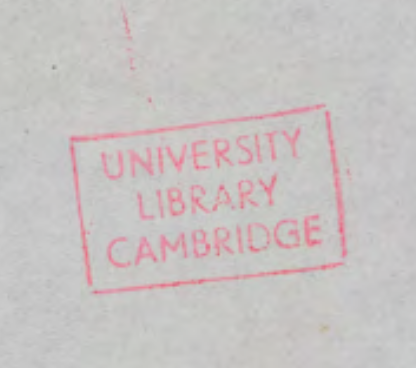
\includegraphics[width=0.23\textwidth]{figures/uni_lib_cambridge.png}
\end{figure}